\chapter{Réalisation et mise en œuvre}
\rhead{Réalisation et mise en œuvre}

%+++++++++++++++++Introduction+++++++++++%
\section{Introduction}


%+++++++++++++++++Outils+++++++++++%
\section{Environnement technique et outils utilisés}
\begin{minipage}{0.7\textwidth}
    \textbf{Visual Studio Code:} est un éditeur de code source qui peut être utilisé avec une variété de langages de programmation, notamment Java, JavaScript, Go, Node.js et C++. Il est basé sur le cadre Electron, qui est utilisé pour développer des applications Web Node.js qui s’exécutent sur le moteur de présentation Blink. Visual Studio Code utilise le même composant d’éditeur (nom de code Monaco) utilisé dans Azure DevOps (anciennement appelé Visual Studio Online et Visual Studio Team Services).
\end{minipage}
\hfill
\begin{minipage}{0.3\textwidth}
    \centering
    
\includegraphics[width=0.4\linewidth]{images/Visual_Studio.png}
    \captionof{figure}{Visual Studio Code}
\end{minipage}

\vspace{1.2cm}

\begin{minipage}{0.7\textwidth}
    \textbf{Snowflake:} est une plateforme de données cloud qui fonctionne comme un entrepôt de données en tant que service (DWaaS). Elle se distingue par une architecture qui sépare le stockage, le calcul et les services de gestion en trois couches indépendantes, permettant de les dimensionner séparément selon les besoins. Snowflake prend en charge les requêtes SQL, les données semi-structurées et offre des fonctionnalités telles que le clonage instantané, le partage de données entre organisations et la réplication multi-cloud.
\end{minipage}
\hfill
\begin{minipage}{0.3\textwidth}
    \centering
    
\includegraphics[width=0.75\linewidth]{images/snowflake.jpg}
    \captionof{figure}{Snowflake}
\end{minipage}

\vspace{1.2cm}

\begin{minipage}{0.7\textwidth}
    \textbf{Cortex:} est un service d'intelligence artificielle intégré nativement à la plateforme Snowflake. Il permet d'exécuter des modèles de langage et de calculer des embeddings vectoriels directement depuis des requêtes SQL, sans que les données ne quittent l'environnement Snowflake
\end{minipage}
\hfill
\begin{minipage}{0.3\textwidth}
    \centering
    
\includegraphics[width=0.7\linewidth]{images/cortex.png}
    \captionof{figure}{Cortex}
\end{minipage}

\vspace{1.2cm}

\begin{minipage}{0.7\textwidth}
    \textbf{Python :} est un langage de programmation interprété, facile à lire et à écrire, connu pour sa simplicité et sa polyvalence. Il est largement utilisé dans de nombreux domaines comme le développement web, l’analyse de données, l’intelligence artificielle, la robotique et l’automatisation. Grâce à sa large communauté et à ses nombreuses bibliothèques, Python est devenu l’un des langages les plus populaires aujourd’hui.
\end{minipage}
\hfill
\begin{minipage}{0.3\textwidth}
    \centering
    
\includegraphics[width=0.5\linewidth]{images/python.png}
    \captionof{figure}{Python}
\end{minipage}

\vspace{1.2cm}

\begin{minipage}{0.7\textwidth}
    \textbf{Streamlit:} est un framework open-source en Python qui permet de créer facilement des applications web interactives pour la data science et le machine learning. Il suffit d’écrire du code Python simple pour transformer des scripts en interfaces web intuitives, sans avoir besoin de connaissances en développement web.
\end{minipage}
\hfill
\begin{minipage}{0.3\textwidth}
    \centering
    
\includegraphics[width=0.5\linewidth]{images/streamlit.png}
    \captionof{figure}{Streamlit}
\end{minipage}

\vspace{1.2cm}

\begin{minipage}{0.7\textwidth}
    \textbf{PowerBI:} est une solution de Business Intelligence développée par Microsoft qui permet de se connecter à diverses sources de données, de les transformer et de les visualiser sous forme de tableaux de bord interactifs. Elle repose sur le langage DAX pour les mesures calculées et le moteur Power Query pour la préparation des données. Power BI offre également un service cloud pour la publication et le partage de rapports au sein d'une organisation.
\end{minipage}
\hfill
\begin{minipage}{0.3\textwidth}
    \centering
    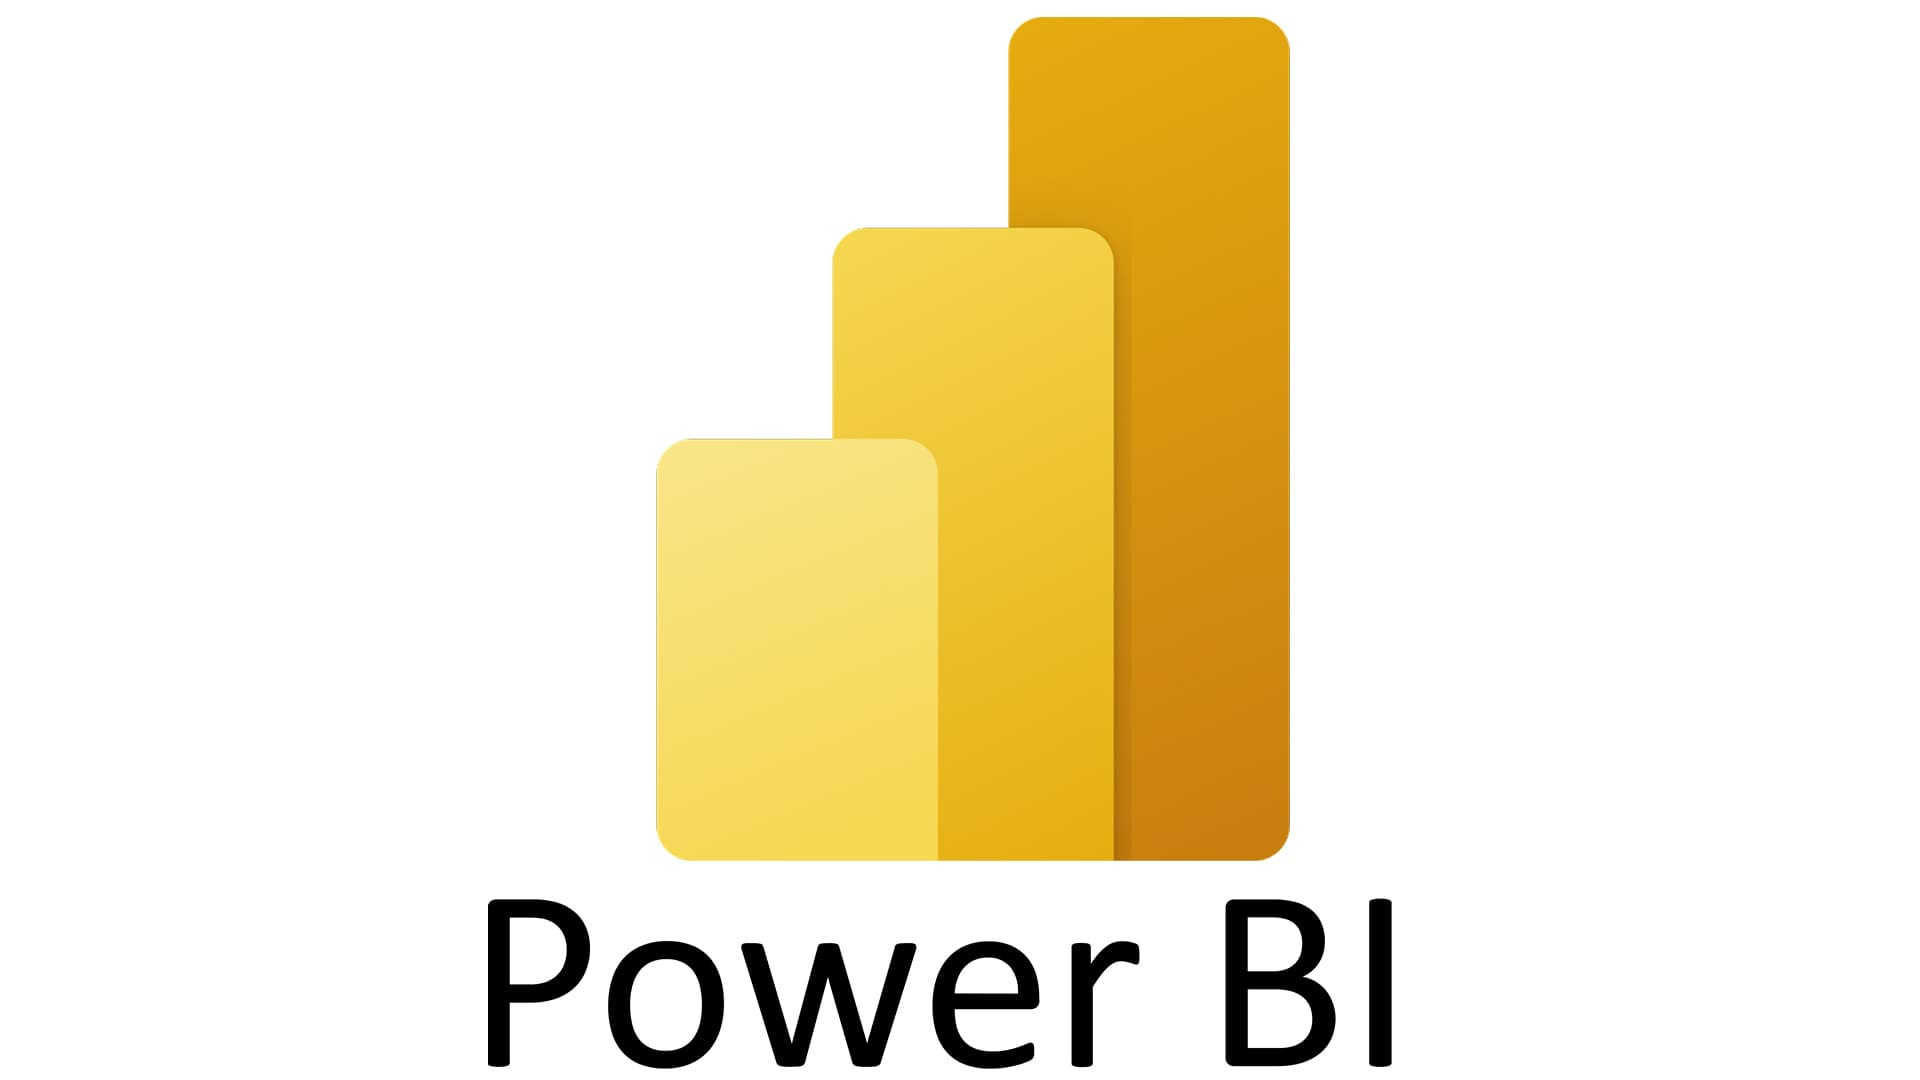
\includegraphics[width=0.7\linewidth]{images/powerbi.jpg}
    \captionof{figure}{PowerBI}
\end{minipage}

\vspace{1.2cm}

\begin{minipage}{0.7\textwidth}
    \textbf{Apache Airflow:} Airflow est un outil open source de gestion et d’orchestration de workflows.
    Il permet de planifier, d’automatiser et de suivre des chaînes complexes de tâches (pipelines de données), en assurant leur exécution dans un ordre précis et en gérant les dépendances entre elles.
\end{minipage}
\hfill
\begin{minipage}{0.3\textwidth}
    \centering
    
\includegraphics[width=0.55\linewidth]{images/airflow.png}
    \captionof{figure}{Airflow}
\end{minipage}


%++++++++++++++++Implémentation+++++++++++%
\section{Implémentation détaillée}


%+++++++++++++++++Resultat+++++++++++%
\section{Tests et validation des résultats}


%+++++++++++++++++Conclusion+++++++++++%
\section{Conclusion}
